
%%%%%%%%%%%%%%%%%%%%%%% file typeinst.tex %%%%%%%%%%%%%%%%%%%%%%%%%
%
% This is the LaTeX source for the instructions to authors using
% the LaTeX document class 'llncs.cls' for contributions to
% the Lecture Notes in Computer Sciences series.
% http://www.springer.com/lncs       Springer Heidelberg 2006/05/04
%
% It may be used as a template for your own input - copy it
% to a new file with a new name and use it as the basis
% for your article.
%
% NB: the document class 'llncs' has its own and detailed documentation, see
% ftp://ftp.springer.de/data/pubftp/pub/tex/latex/llncs/latex2e/llncsdoc.pdf
%
%%%%%%%%%%%%%%%%%%%%%%%%%%%%%%%%%%%%%%%%%%%%%%%%%%%%%%%%%%%%%%%%%%%


\documentclass[runningheads,a4paper]{llncs}
\bibliographystyle{splncs03}

\usepackage{amssymb}
\setcounter{tocdepth}{3}
\usepackage{graphicx}
\usepackage[utf8]{inputenc}

\usepackage{color}
\usepackage{url}
\usepackage{amsmath}
\usepackage[colorinlistoftodos,prependcaption,textsize=small]{todonotes}

\usepackage[titletoc, title]{appendix}
\usepackage[ruled]{algorithm}
\usepackage{algpseudocode}

% to increase the spacing between the caption and the table
\usepackage{caption}
\captionsetup[table]{skip=10pt}

\newcommand{\keywords}[1]{\par\addvspace\baselineskip
\noindent\keywordname\enspace\ignorespaces#1}

\raggedbottom
\pagestyle{plain}

\begin{document}

\mainmatter  % start of an individual contribution

% first the title is needed
\title{Replication with variable consistency and tolerance to arbitrary uncorrelated faults}

\author{Miguel Pires \\
\texttt{miguel.pires@tecnico.ulisboa.pt}}

% (feature abused for this document to repeat the title also on left hand pages)

% the affiliations are given next; don't give your e-mail address
% unless you accept that it will be published
\institute{Instituto Superior Técnico (Campus Taguspark) \\
Av. Prof. Doutor Aníbal Cavaco Silva \\
2744-016 Porto Salvo - Portugal}

%
% NB: a more complex sample for affiliations and the mapping to the
% corresponding authors can be found in the file "llncs.dem"
% (search for the string "\mainmatter" where a contribution starts).
% "llncs.dem" accompanies the document class "llncs.cls".
%

\let\oldaddcontentsline\addcontentsline
\def\addcontentsline#1#2#3{}
\maketitle
\def\addcontentsline#1#2#3{\oldaddcontentsline{#1}{#2}{#3}}

%\toctitle{Replication with variable consistency and tolerance to arbitrary uncorrelated faults}
%\tocauthor{Authors' Instructions}
%\maketitle

\begin{abstract}
Generalized consensus is a generalization of traditional consensus that allows us to define problems that take advantage of commutative operations to reduce coordination requirements when committing values. However, the specifications of both generalized consensus and the protocol that solves it, Generalized Paxos, are complex and not widely understood. We propose to do a thorough study of this problem by solving it in a broad system model that allows for different synchrony and fault tolerance configurations, the Visigoth model. This report surveys related work and presents preliminary results. Among these results is a concise description of the Generalized Paxos protocol that is simpler than what was originally presented and which will be used as a starting point for the remaining work. We also describe how this protocol can be extended to support Byzantine fault tolerance and present some results regarding the transformation of fast quorums to the Byzantine model. Additionally, we describe what future works remains and how we intend to complete it.

\keywords{Generalized Consensus, Generalized Paxos, Fault Tolerance, Visigoth Model}
\end{abstract}

\newpage
\tableofcontents
\newpage

\section{Introduction}
\subsection{Motivation}
The consensus problem requires that processes agree on proposed values in the presence of $f$ faults and its solution has been essential to solve many distributed computing problems. One of the most important contributions to this field is the Fischer, Lynch and Patterson (FLP) impossibility result that states that the consensus problem is unsolvable in an asynchronous system even if only one process can fail \cite{Fischer1985}. Lamport's Paxos algorithm is able to solve consensus, circumventing the FLP impossibility result, by ensuring that values are always safely decided while progress is only guaranteed when the system is synchronous for a sufficient amount of time \cite{Lamport2001}. In Paxos, there are 3 types of processes: \textit{proposers}, which propose values to be committed; \textit{acceptors}, which vote on proposed values; and \textit{learners}, that learn values voted on by a quorum of acceptors (i.e., committed). This problem has gone from a theoretical exercise to a fundamental part of many large-scale, modern distributed systems such as Google's Chubby \cite{Burrows2006}, Spanner \cite{Corbett2012} and Apache's ZooKeeper \cite{Junqueira2011}. These systems power services like the Google Search Engine, using techniques like state machine replication (SMR) to allow them to remain highly available even in the presence of faults and asynchronous communication channels. \par
Generalized consensus is a generalization of traditional consensus that abstracts the problem of agreeing on a single value to a problem of agreeing on a monotonically increasing set of values. This problem is defined in terms of a set of values called command structures, \textit{c-structs} \cite{Lamport2005}. These structures allow for the formulation of different consensus problems, including consensus problems where commutative operations are allowed to be ordered differently at different replicas (i.e., command histories). The advantage of such a problem can be seen in Fast Paxos, where fast ballots are executed by having proposers propose directly to acceptors \cite{Lamport2006}. By avoiding sending the proposal to the leader, values can be learned in the optimal number of two message delays. However, if two proposers concurrently propose different values to acceptors, a conflict arises and at least an additional message delay is required for the leader to solve it. This is the cost that Fast Paxos pays in order to commit values in a single round trip.  Generalized consensus allows us to reduce this cost, if we define the problem as one of agreeing on command histories. Since histories are considered equivalent if non-commutative operations are totally ordered, the only operations that force the leader to intervene are non-commutative ones. An additional advantage of the generalized consensus formulation stems from its generality and from the fact that we can use the Generalized Paxos protocol to solve it despite its high level of abstraction. This protocol can be used to solve any consensus problem that can be defined in terms of generalized consensus, not only the command history problem. The reason why Generalized Paxos can take advantage of the possibility of reordering commutative commands is that it allows acceptors to accept different but compatible \textit{c-structs}. Two \textit{c-structs} are considered to be compatible if they can later be extended to equivalent \textit{c-structs}. In command histories, if all non-commutative commands are totally ordered, then two \textit{c-structs} are considered equivalent. \par
One application of the generalized consensus specification can be to implement SMR using command histories to agree on equivalent sequences of operations. For instance, consider a system with four operations $\{A, B, C, D\}$ where $C$ and $D$ are non-commutative. If two proposers concurrently propose the operations $A$ and $B$, some acceptors could accept $A$ first and then $B$ and other acceptors could accept the operations in the inverse order. However, this would not be considered a conflict and the leader wouldn't have to intervene since the operations commute. If two proposers tried to commit $C$ and $D$, acceptors could accept them in different orders which would be considered a conflict since these operations are non-commutative. In this situation, no \textit{c-struct} would be chosen and the leader would be forced to intervene by initiating a higher-numbered ballot to commit either $w \bullet C \bullet D$ or $w \bullet D \bullet C$. It's important to note that this is only one possible application of the Generalized Paxos protocol and that this protocol solves any problem that can be defined by the generalized consensus specification. \par
The approach of allowing the system to reorder operations may feel familiar to the reader, since it resembles how weak consistency models relax consistency guarantees to allow replicas to reorder operations \cite{Ladin1992}. By relaxing consistency and allowing operations to be reordered, these models reduce coordination requirements which results in decreased latency and better operation concurrency. However, relaxing consistency guarantees also introduces the chance of state divergence which can be tolerable or not depending on the application. These approaches are critical to geo-replicated scenarios where it's important to reduce round trips between data centers and maintaining strong consistency incurs in an unacceptable latency cost. \par
The Paxos protocol family has been a subject of study for some time, due to its importance in the area of consensus and state machine replication. Recent work in this area includes Mencius \cite{Mao2008} and EPaxos \cite{Moraru2013}, which try to increase throughput by eliminating the bottleneck caused by having a single leader that sends proposals to acceptors. The Generalized Paxos protocol is similar to these approaches in the sense that it also decreases the load put on the leader by allowing proposers to bypass it. However, despite generalized consensus' potential, it's still an understudied problem and its formulation is rather complex and abstract which makes it hard to understand and reason about. This complexity also makes the algorithm hard to implement and adapt to different scenarios. A symptom of this is that only the original Generalized Paxos protocol exists for this problem and few works make use of it.  \par
Another consequence of the lack of knowledge about generalized consensus is that there are several potentially interesting research questions that researchers haven't answered. For instance, despite the connection between the commutativity observation that motivated generalized consensus and the reduced coordination requirements made possible by weak consistency, it is unclear how Generalized Paxos would function in geo-replicated scenarios where the goal is to minimize cross-datacenter round trips. The goal of Generalized Paxos is to reduce communication steps without requiring a leader to solve conflicts that emerge from concurrently executed operations but few works have tried to align this algorithm with a multi-datacenter scenario. Similarly, there is no research on what effects the Byzantine assumption would have on the solution of the generalized consensus problem.
\par

\subsection{Expected Contribution}
The goal of this work is to perform a thorough study of the generalized consensus problem to gain a deeper knowledge about the applicable protocols and how they behave in different scenarios. This will enable us to explore previously unanswered avenues of research, such as the adaptation of generalized consensus protocols for the Byzantine assumption. To perform this study, we will use a broad and generic system model called the Visigoth model \cite{Porto2015}. Using this model, a system can be parametrized to allow for any amount of synchrony, ranging from full asynchrony to full synchrony. Similarly, the system administrator can also specify any amount of Byzantine or crash faults, allowing the system to support any combination of faults within the spectrum between crash and Byzantine faults. With this model we can study generalized consensus from different perspectives and propose a solution that allows generalized consensus to be solved across a broad spectrum of system models. \par 
Since the generalized consensus formulation is very intricate and hard to understand, we will also propose a simpler formulation for generalized consensus. This will allow us to better reason about this problem while still preserving its usefulness. We will focus on the command history problem where \textit{c-structs} are considered equivalent if all non-commutative operations are totally ordered. This specialization of the generalized consensus problem allows us to take advantage of the specification without the added complexity implied by the original specification's generality. \par
By solving generalized consensus in the Visigoth model, we expect to obtain a protocol that can be used in different instantiations of the model. One particularly interesting application is similar to that of weakly consistent systems, geo-replicated datacenters. By specifying a consensus problem akin to command histories, our protocol could take advantage of operation commutativity to minimize the number of ballots that incur in a higher coordination cost. In this scenario, the parameterizability of Visigoth model also plays an important role since we can specify a number of slow processes that allows us to reduce the number of replicas that are required to safely commit values. Another potentially interesting scenario, related to the fault model, could be one where we tolerate arbitrary, uncorrelated faults. This is an interesting scenario since it's enough to deal with arbitrary state corruption faults, which are common within datacenters \cite{AmazonS32}, but avoids the cost of dealing with coordinated Byzantine behavior.

\subsection{Document Outline}

The remainder of this document is structured as follows: Section 2 is divided in five subsections and surveys works that are related to our own and may provide relevant insights into the problem we're trying to solve. Each subsection describes scientific works in a specific area of interest to us. Section 3.1 describes what we have accomplished so far regarding the solution to generalized consensus in the Visigoth model. Section 3.2 proposes how these preliminary results should be extended to arrive at the final solution. Section 3.3 describes how the developed solution will be validated. Section 3.4 proposes a schedule for the development, implementation, validation and documentation of future work.

\section{Related Work} \label{Related Work}

Due to the specific characteristics of both the problem that we wish to solve and the system model in which it will be solved, there are several areas that contain works of interest to us. Subsection \ref{Paxos} describes previous work regarding consensus and several Paxos variants. Subsection \ref{Non-Crash} discusses non-crash fault models as well as protocols for that solve consensus in these environments. Subsection \ref{Partial Synchrony} describes different partial synchrony models and how they fit in the synchrony spectrum. Subsection \ref{Variable Consistency} discusses variable consistency models that attempt to strike a balance between strong and weak consistency in order to obtain advantages from both. Despite the fact that the Paxos protocol family has been a subject of study for some time, this topic is now more relevant than ever since modern systems use these algorithms to implement high-availability, large scale systems. Subsection \ref{Coordination Systems} studies a few systems where these algorithms are used to enable fault-tolerance services.

\subsection{Paxos and its Variants} \label{Paxos} 

The Paxos protocol family solves consensus by circumventing the well-known FLP impossibility result \cite{Fischer1985}. It does this by making the observation that, while consensus is unsolvable in asynchronous systems, most of the time systems can be considered synchronous since delays are sporadic and temporary. Therefore, as long as consistency is guaranteed regardless of synchrony, Paxos can forgo of progress during the temporary periods of asynchrony. Using this insight, Paxos ensures consistency even when the system is asynchronous but can only guarantee progress while it is synchronous and no more than $f$ faults occur for a system of $2f+1$ replicas \cite{Lamport2001}. The classic form of Paxos employs a set of proposers, acceptors and learners and runs in a sequence of ballots. To ensure progress during synchronous periods, proposals are serialized by a distinguished proposer, the leader. It is the leader that gathers proposals from other proposers and requests, in a \textit{phase 1a} message, that acceptors promise to not accept any ballots smaller than its own. Each acceptor responds to the leader's request, in a \textit{phase 1b} message, with either a promise or a message stating that it has already sent a promise to a proposer with a higher-numbered ballot. If the leader manages to obtain a promise from a quorum of acceptors, then it sends a \textit{phase 2a} message containing its proposal. The acceptors may accept the proposal and inform the learners with a \textit{phase 2b} message, if another proposer hasn't requested a promise for a higher-numbered ballot in the meanwhile. The fact that any proposer can request a promise and prevent lower ballots from being completed is the reason why Paxos can only ensure progress in a synchronous environment. Some proposer must be able to establish itself as the only leader in order to prevent proposers from continuously requesting promises for ballots with higher numbers. \par
We now describe the form in which Paxos is most commonly deployed, Multi(Decree)-Paxos. Multi-Paxos provides an optimization of the basic Paxos' message pattern by omitting the first phase of messages from all but the first ballot for each leader \cite{Renesse2011}. This means that a leader only needs to send a \textit{phase 1a} message once and subsequent proposals may be sent directly in \textit{phase 2a} messages without requesting a promise from the acceptors. This reduces the message pattern in the common case from five message delays to just three (from proposal to learning). Since there are no implications on the quorum size or guarantees provided by Paxos, the reduced latency comes at no additional cost. \par
Fast Paxos observes that it's possible to improve on previous results by allowing proposers to propose values directly to acceptors. To this end, the protocol distinguishes between fast and classic ballots, where fast ballots bypass the leader by sending proposals directly to acceptors and classic ballots work as in Basic Paxos. The fast ballots' reduced latency comes at the additional cost of using a quorum size larger than $\frac{3N}{4}$ instead of a classic majority quorum. Additionally, $N$ must be larger than $2e+f$  where $f$ is the number of faults that can be tolerated while still using classic ballots and $e$ is the number of faults that can be tolerated while using fast ballots. For instance, if we wish to tolerate the same number of faults for classic and fast ballots (i.e., $e=f$),. then the total number of replicas is $3f+1$ instead of the usual $2f+1$. The optimized scenario occurs during fast ballots, in which only two messages broadcasts are necessary: \textit{phase 2a} messages between a proposer and the acceptors, and \textit{phase 2b} messages between acceptors and learners. This creates the possibility of two proposers concurrently proposing values to the acceptors and generating a conflict. The cost of dealing with this conflict depends on the chosen method of recovery, coordinated or uncoordinated, and if the leader or acceptors are also learners. The leader may choose  the recovery method in the beginning of the ballot. If coordinated recovery is chosen in a ballot $i$, then the cost is a \textit{phase 2} of round $i+1$ (i.e., two additional message delays). If uncoordinated recovery is chosen then the cost is a single \textit{phase 2b} message in round $i+1$ (i.e., one message delay) \cite{Lamport2006}. These numbers assume that either the leader (coordinated recovery) or the acceptors (uncoordinated recovery) are learners, which is a reasonable assumption. \par
Generalized Paxos addresses Fast Paxos' shortcomings regarding collisions. More precisely, it allows acceptors to accept different sequences of commands as long as non-commutative operations are totally ordered \cite{Lamport2005}.  Non-commutativity between operations is generically represented as an interference relation. Generalized Paxos abstracts the traditional consensus problem of agreeing on a single value to the problem of agreeing on an increasing set of values. \textit{C-structs} provide this increasing sequence abstraction and allow us to define different consensus problems. If we define the sequence of learned commands of a learner $l_i$ as a \textit{c-struct} $learned[l_i]$, then the consistency requirement for consensus can be defined as:\par
\textbf{Consistency} $learned[l_1]$ and $learned[l_2]$ are always compatible, for all learners $l_1$ and $l_2$. \par
For two \textit{c-structs} to be compatible, they must have a \textit{common upper bound}. This means that, for any two learned \textit{c-structs} such as $learned[l_1]$ and $learned[l_2]$, there must exist some \textit{c-struct} to which they are both prefixes. This prohibits non-commutative commands from being concurrently accepted because no subsequent \textit{c-struct} would extend them both since it wouldn't have a total order of non-commutative operations. For instance, consider a set of commands $\lbrace A$, $B$, $C\rbrace$ and an interference relation between commands $A$ and $B$ (i.e., they are non-commutative with respect to each other). If clients propose $A$ and $C$, some learners may learn one command before the other and the resulting \textit{c-structs} would be either $C \bullet A$ or $A \bullet C$. These are compatible because there are \textit{c-structs} that extend them, namely $A \bullet C \bullet B$ and $C \bullet A \bullet B$. These \textit{c-structs} that extend them are valid because the interfering commands are totally ordered. However, if two clients propose $A$ and $B$, learners could learn either one in the first ballot and these \textit{c-structs} would not be compatible because no \textit{c-struct} extends them. Any \textit{c-struct} would start either by $A \bullet B$ or $B \bullet A$, which means that an interference relation would be violated. In the Generalized Paxos protocol, when such a collision occurs, no value is chosen and the leader intervenes by starting a new ballot and proposing a \textit{c-struct}. Defining \textit{c-structs} as command histories enables acceptors to agree on different sequences of commands and still preserve consistency as long as dependence relationships are not violated. This means that commutative commands can be ordered differently regarding each other but interfering commands must preserve the same order across each sequence at any learner. This guarantees that solving the consensus problem for histories is enough to implement a state-machine replicated system. \par
Multi-Data Center Consistency (MDCC) is an optimistic commit protocol that uses Generalized Paxos for transaction processing. MDCC uses fast commutative ballots to commit several commutative updates in the same ballot with potentially different orders across storage nodes \cite{Kraska2013}. To preserve global constraints (e.g., the stock should never go below zero), a demarcation technique is used to limit the amount of transactions that can be committed in a ballot. MDCC is one of the few works that takes advantage of Generalized Paxos to concurrently commit commutative operations.\par
Mencius is also a variant of Paxos that tries to address the bottleneck of having a single leader through which every proposal must go through. In Mencius, the leader of each round rotates between every process. The leader of round $i$ is the process $p_k$, such that $k = n\ mod\ i$.  Leaders with nothing to propose can skip their turn by proposing a \textit{no-op}. If a leader is slow or faulty, the other replicas can execute \textit{phase 1} to revoke the leader's right to propose a value but they can only propose a \textit{no-op} instead \cite{Mao2008}. Considering that non-leader replicas can only propose \textit{no-ops}, a \textit{no-op} command from the leader can be accepted in a single message delay since there is no chance of another value being accepted. If some non-leader server revokes the leader's right to propose and suggests a \textit{no-op}, then the leader can still suggest a value $v \neq$ \textit{no-op} that will eventually be accepted as long as $l$ isn't permanently suspected. The usage of an unreliable failure detector is enough to guarantee that eventually all faulty processes, and only those, will be suspected. Mencius also takes advantage of commutativity by allowing out-of-order commits, where values $x$ and $y$ can be learned in different orders by different learners if there isn't a dependence relationship between them. Experimental evaluation confirms that Mencius is able of scaling to a higher throughput than Paxos. \par
Egalitarian Paxos (EPaxos) extends Mencius' goal of achieving a better throughput than Paxos by removing the bottleneck caused by having a leader. Additionally, EPaxos also achieves optimal commit latency in certain conditions and graceful performance degradation if replicas fail or become slow \cite{Moraru2013}. To avoid choosing a leader, the proposal of commands for a command slot is done in a decentralized manner. Each replica can propose a command with ordering constraints attached so that interfering commands can be totally ordered. In this way, EPaxos takes advantage of the commutativity observations made by Generalized Paxos that state that commutative commands may be ordered differently at different replicas without losing state convergence \cite{Lamport2005}. If two replicas unknowingly propose commands concurrently, one will commit its proposal in one round trip after getting replies from a quorum of replicas. However, some replica will see that another command was concurrently proposed and may interfere with the already committed command. If the commands are commutative then there is no need to impose a particular order but, if they're not commutative, then the replica must reply with a dependency between the commands. If a replica commits a command $A$ in a single round trip, then the replica that tries to concurrently propose a non-commutative command $B$ would receive a reply with the ordering $B \rightarrow \{A\}$, to indicate that $B$ should be committed after $A$. In this scenario, committing command $B$ would require two round trips since the proposer would need to send another message to inform the other replicas of the new ordering constraint. This commit latency is achieved by using a \textit{fast-path quorum} of $f+\lfloor\frac{f+1}{2}\rfloor$ replicas which is the same as the \textit{slow-path quorum} of $f+1$ replicas, for $f \leq 2$. Similarly to Mencius, EPaxos achieves a substantially higher throughput than Multi-Paxos, especially when $2\%$ of commands interfere with each other. However, since, unlike Mencius, replicas don't have to wait for previous replicas to propose their commands, commit latency is significantly lower.

\subsection{Non-crash Fault Models} \label{Non-Crash}
Non-crash fault models emerged to cope with the effect of malicious attacks and software errors. These models (e.g., the arbitrary fault model) assume a stronger adversary than previous crash fault models. The Byzantine Generals Problem is defined as a set of Byzantine generals that are camped in the outskirts of an enemy city and have to coordinate an attack. Each general can either decide to attack or retreat and there may be $f$ traitors among the generals that try to prevent the loyal generals from agreeing on the same action. The problem is solved if every loyal general agrees on what action to take \cite{Lamport1982}. Like the traitorous generals, the Byzantine adversary is one that may force a faulty replica to display arbitrary behaviour and even coordinate multiple faulty replicas in an attack. It's interesting to survey non-crash fault models since we intend to explore the effects that different models have on the solutions for the generalized consensus problem. \par
PBFT is a protocol that solves consensus for state machine replication while tolerating up to $f$ Byzantine faults \cite{Castro1999}. The system moves through configurations called \textit{views} in which one replica is the primary and the remaining replicas are the backups. The safety property of the algorithm requires that operations be totally ordered. The protocol starts when a client sends a request for an operation to the primary, which in turn assigns a sequence number to the request and multicasts a \textit{pre-prepare} message to the backups. This message contains the timestamp, the message's digest, the view and the actual message. If a backup replica accepts the pre-prepare message, after verifying that the view number and timestamp are correct, it multicasts a \textit{prepare} message and adds both messages to its log. The prepare message is similar to the pre-prepare message except that it doesn't contain the client's request message. Both of these phases are needed to ensure that the requested operation is totally ordered at every correct replica. The protocol's safety property requires that the replicated service must satisfy linearizability, and therefore operations must be totally ordered. After receiving $2f$ prepare messages, a replica multicasts a \textit{commit} message and commits the message to its log when it has received $2f$ commit messages from other replicas. The liveness property requires that clients must eventually receive replies to their requests, provided that there are at most $\lfloor\frac{n-1}{3}\rfloor$ faults and the transmission time doesn't increase continuously. This property represents a weak liveness condition but one that is enough to circumvent Fischer, Lynch and Paterson's impossibility result \cite{Fischer1985}. A Byzantine leader may try to prevent progress by omitting pre-prepare messages when it receives operation requests from clients, but backups can trigger new views after waiting for a certain period of time. \par
The cost of $3f+1$ replicas in a PBFT system stems from the immense power given to the adversary. The cross fault tolerance (XFT) model claims that this adversary is too strong when compared to the behavior of deployed systems \cite{Liu2015}. XFT assumes that machine and network faults are uncorrelated and this assumption allows it to have a cost equal to crash fault tolerant systems, $2f+1$, while still tolerating $f$ non-crash faults. The safety condition for this model is that correct replicas commit requests in a total order, as long as the system is not in anarchy. A system is in anarchy if there are any non-crash faults $f_{nc}(s)$ and the sum of crash faults $f_c(s)$, non-crash faults $f_{nc}(s)$ and partitioned replicas $f_p(s)$ is larger than the fault threshold. That is, the system is in anarchy if $f_{nc}(s) > 0\ \land\ f_{nc}(s)+ f_c(s)+f_p(s) > f$. Liveness is also guaranteed as long as the system is outside of anarchy. XFT replicates client requests to $f+1$ replicas synchronously while the remaining $f$ may learn about requests through lazy replication \cite{Ladin1992}. If an active replica fails, a view change is triggered. A view change requires all the replicas in the new view to collect the recent state, including the commit log, which may be substantial. This overhead can be decreased through the use of checkpointing. The protocol includes the exchange of four rounds of messages: SUSPECT, VIEW-CHANGE, VC-FINAL and NEW-VIEW. The experimental evaluation performed by the authors shows that, after each crash, the system triggers a view change that last less than 10 seconds. \par
The creators of the Visigoth Fault Tolerance (VFT) model also make the observation that the Byzantine model is unrealistic, especially for environments such as data centers. The Byzantine adversary's strength forces protocols to incur in an unnecessary cost of $3f+1$ replicas. VFT also notes that while data centers rarely observe arbitrary coordinated faults, they commonly experience data corruption faults (e.g., bit flips) and these also represent a type of arbitrary behaviour \cite{AmazonS31}\cite{AmazonS32}. To reconcile the need to tolerate different types of arbitrary faults, VFT observes that it is very unlikely for data corruption to affect the same data across multiple replicas. Therefore, the key distinguishing factor between these types of arbitrary faults is \textit{correlation}. VFT proposes a customizable model that defines a limit of $u$ faults, that bounds the number of allowed omission (i.e., crash) and comission (i.e., arbitrary) faults, a limit of $o$ correlated comission faults, a limit of $r$ arbitrary faults and, for every process $p_i$, $s$ correct processes $p_j$ that are slow with respect to it \cite{Porto2015}. These additional assumptions allow the Visigoth model to decrease the replication factor from $n \geq 2u+r+1$ (i.e., $3f+1$ in the traditional notation) to $n \geq u+s+o+1$ (i.e., $f+s+o+1$), when $u > s$. These parameters allow the system administrator to configure the system to tolerate any combination of faults. The authors also propose a VFT state machine replication protocol, which is adapted from the BFT-SMaRt protocol and contains two main message patterns: the first consists in two message steps that are executed during epoch changes to collect information about previous epochs and disseminate this information to replicas; and the second consists in two multicast phases that are executed for each client request to implement the state machine replication. To gather a quorum, the gatherer tries to collect a larger quorum of $n-s$ replies, which can be seen as collecting replies from the fast but potentially faulty replicas. If a timeout occurs, the quorum is reduced to $n-u$ and this can be seen as collecting replies from correct but possibly slow replicas. This reduced quorum size is enough to ensure an intersection because since $x$ replicas didn't reply by the first timeout and only $s$ may be slow, then $x-s$ replicas must have crashed and won't participate in future quorums. The experimental evaluation confirms that VFT can tolerate uncorrelated arbitrary faults with resource-efficiency and performance that resembles that of CFT systems instead of BFT. \par
Dijkstra proposed self-stabilizing systems as a solution to the problem of keeping cyclic sequences of processes in a legitimate state even after the occurrence of transient faults \cite{Dijkstra1974}. In a self-stabilizing system, each process may contain several privileges and may only exchange information with its neighbors. The requirement of keeping the system in a legitimate state is met if: (1) one or more privileges are present; (2) in each state, the possible moves transfer the system to a legitimate state again (3) each privilege exists in at least one legitimate state; and (4) for any pair of legitimate states, there is a sequence of moves that transfers the system from one to the other. These systems define a set of rules for transferring privileges in a way such that a system that starts from an arbitrary state is guaranteed to converge to a legitimate state and remain in a set of legitimate states. Self-stabilizing systems are an example of a non-crash model that isn't strictly stronger than crash fault models since, due to the system's ring-like structure, a crash fault would render the system unusable. A self-stabilizing system tolerates any arbitrary corruption of the state but, unlike other non-crash models, it assumes that a process always executes correct code.\par
The Arbitrary State Corruption (ASC) model defines ASC faults as faults that occur at a process $p$ and either make it crash or assign an arbitrary value to a variable of the process's state. The assignment of an arbitrary value to a variable of $p$'s state may also alter its control flow in a way such that the process may execute any of its instructions \cite{Correia2012}. This modeling stems from three main observations: (1) most tolerable failures are caused by state corruptions instead of arbitrary or malicious behavior, (2) control-flow faults are very likely to cause incorrect outputs \cite{Kalbarczyk2003}, and (3) the relevant failures are caused by transient faults instead of permanent faults being repeatedly activated. In the context of this model, the ASC hardening technique is proposed to deal with ASC faults. This technique guarantees that, if a correct hardened process $p_c$ receives a message $m$ from a faulty hardened process $p_{f1}$, then $p_c$ discards $m$ without modifying its state. If a faulty process $p_{f2}$ receives $m$ and modifies its local state, then it crashes before sending an output message. ASC hardening uses message integrity checks to prevent network corruption and state integrity checks to replicate process state. Every time a value is read from a variable, it's checked against the replicated value. If a mismatch occurs, the process crashes itself to preserve integrity. Control-flow faults are prevented through the use of gates, which are sequences of instructions that ensure that a portion of code is executed the appropriate number of times. For instance, we may want to ensure that an event handler executes exactly once per event. For each control-flow gate, two variables and a label are created, respectively, $c$, $c'$ and $L$. A gate executes a sequence of checks and assignments to ensure the required semantics. A useful type of control-flow gate is an \textit{at-most-once} gate, which ensures that code isn't executed twice even in the presence of faults. An \textit{at-most-once} gate implements these semantics by crashing the process if $c \neq c' \vee c=L$. In the first execution of the code, the condition fails, both $c$ and $c'$ are set to $L$ and the execution continues. In a second execution, the condition would evaluate to true since $c$ has already been set to $L$ and the process would crash. The $c \neq c'$ condition prevents an arbitrary state fault from corrupting the variable's value. Another relevant type of control-flow gate is an \textit{at-least-once} gate, which ensures that a gate has been executed before. For an \textit{at-least-once} gate, if $c=c'=L$ the gate has been reached before. Otherwise, the process crashes itself. ASC is similar to self-stabilizing systems \cite{Dijkstra1974} in the sense that both assume that only state can become corrupted, while the executed code is always correct. An ASC-hardened implementation of Paxos has a throughput up to 70\% higher than PBFT. \par
Zeno is Byzantine fault tolerance state machine replication protocol that favors availability instead of consistency \cite{Singh2009}. By trading strong consistency for eventual consistency, Zeno provides higher availability when networks partitions occur and better performance when replica latency is heterogeneous.  A client request is said to be \textit{weakly complete} if the client gathers matching replies from a \textit{weak quorum} of $f+1$ replicas. This ensures the client that at least one correct replica will execute the request and commit it to the linear history. For a request to be \textit{strongly complete}, the client must wait for matching replies from a \textit{strong quorum} of $2f+1$ replicas. In the case of a partition, two clients concurrently issuing requests may cause divergent histories that can later be merged to restore consistency between replicas. When a replica receives a client request, it performs the appropriate security checks (e.g., message authenticity, correct view, etc) and executes the requested operation. If the request was for a weak operation, the replica replies to the client immediately after the operation terminates. However, if the request was for a strong operation, the replica multicasts a \textit{COMMIT} message to the other replicas and waits for $2f$ matching messages. After receiving $2f$ \textit{COMMIT} messages, the replica forms a commit certificate for the messages it received, stores it and replies to the client. To further increase availability, Zeno's view change protocol is also guaranteed to proceed with only a weak quorum of replicas. Strongly consistent BFT systems require view change protocols to gather a strong quorum to ensure that a view change quorum intersects in at least one correct replica with any other quorum. If this property isn't ensured, another quorum could commit a request that would be unseen by the view change. In Zeno, a request can go unnoticed by view change quorum, resulting in divergent histories and a subsequent merge. \todo{Is this enough or should I go into divergence detection and merger?}

\subsection{Partial Synchrony} \label{Partial Synchrony}
The design of the Paxos protocol is based on the observation that, although it's possible to guarantee safety in a fully asynchronous environment, a system can only ensure liveness when the network behaves synchronously for a sufficient amount of time \cite{Lamport2001}. Therefore, it makes sense for us to study the effects that different synchrony assumptions, such as partial synchrony, have on the consensus problem and on the algorithms that solve it. Additionally, the Visigoth model allows for a configurable amount of synchrony to be tolerated by the system, which makes it even more relevant for us to study its effects \cite{Porto2015}. \todo{Is this ok? If not, what's my "motivation" for this section? Does the phrasing sound strange?} \par
A failure detector is a formalism that allows us to abstract the assumptions a system is allowed to make about its environment. Unreliable failure detectors were proposed by Chandra and Toueg as a way to circumvent impossibility results due to asynchrony. These failure detectors would output information about which processes have crashed, therefore encapsulating the necessity of determining whether a process is crashed or slow \cite{DeepakChandra1996}. The guarantees provided by the failure detector are specified in terms of \textit{completeness}, which requires that a failure detector must eventually suspect every crashed process, and \textit{accuracy}, which restricts the mistakes a failure detector can make. A class of failure detectors of particular interest is Eventually Weak failure detectors, $\Diamond\mathcal{W}$, since it is the weakest of all classes defined by Chandra and Toueg. $\Diamond\mathcal{W}$ failure detectors provide the following guarantees:\par
\textbf{Completeness} Eventually every crashed process is permanently suspected by some correct process.\par
\textbf{Accuracy} Eventually some correct process is never suspected by any correct process.\par
Chandra and Toueg prove that consensus is solvable using a $\Diamond\mathcal{W}$ failure detector with $f < \lceil n/2 \rceil$ \cite{DeepakChandra1996}. Chandra et al. also define a new class of failure detectors, $\Omega$-accurate failure detectors \cite{Chandra1996}. The $\Omega$ class is shown to be at least as strong as $\Diamond\mathcal{W}$ and any failure detector that allows consensus to be solved must be at least as strong as $\Omega$. Therefore, any failure detector that allows consensus to be solved is at least as strong as $\Diamond\mathcal{W}$ which is then the weakest possible class of failure detector with which consensus can be solved. \par
The accuracy properties of the failure detectors proposed by Chandra and Toueg in \cite{DeepakChandra1996} must apply to all processes in the system. If a network partition occurs, the accuracy property can be violated since correct processes in one partition may be suspected to have failed by processes in a different  partition. $\Gamma$-accurate failure detectors were proposed by Guerraoui and Schiper \cite{Guerraoui96gammaaccurate} to deal with this limitation in the specification of $\Omega$-accurate failure detectors. $\Gamma$-accurate failure detectors apply the completeness and accuracy properties to a subset of the system's processes and allow consensus to be solved in a fully asynchronous model. The accuracy property for a $\Gamma$-accurate Eventually Weak failure detector, $\Diamond\mathcal{W}(\Gamma)$, becomes: \par
\textbf{Accuracy} Eventually some correct process (not necessarily in $\Gamma$) is never suspected by any process in $\Gamma$.\par
Since $\Gamma$-accurate Eventually Weak failure detectors are strictly weaker than $\Omega$-accurate Eventually Weak failure detectors \cite{Guerraoui96gammaaccurate}, $\Diamond\mathcal{W}(\Gamma) \prec \Diamond\mathcal{W}$, and  $\Diamond\mathcal{W}$ failure detectors have been shown to be the weakest class of failure detectors for which consensus is solvable \cite{Chandra1996}, then it follows that $\Diamond\mathcal{W}(\Gamma)$ failure detectors do not allow for consensus to be solved.\par
Wide-area systems are often considered to be asynchronous since they cannot provide a fixed upper bound $\Delta$ on the time messages take to be delivered (communication synchrony) or a fixed upper bound $\Phi$ on the drift rate between processes' clocks (process synchrony). However, Dwork, Lynch and Stockmeyer note that one reasonable situation is when there exists an upper bound $\Delta$ on message delivery latency but it isn't known \textit{a priori} \cite{Dwork1988}. In a realistic deployment, a system could consider the network to be synchronous for most of the time since connectivity and network problems are sporadic. In this situation, the impossibility results shown in \cite{Fischer1985} and \cite{Dolev1983} don't apply since communication can be considered synchronous. To take advantage of an existent but unknown upper bound $\Delta$ on communication time, a consensus-solving protocol can't explicitly use $\Delta$ as a timeout value because it's unknown. Additionally, for this protocol to progress, there should be a time after which this upper bound holds. Therefore, an additional constraint is applied to the model: there is a global stabilization time (GST) after which communication latency is bounded by $\Delta$. An algorithm that solves consensus is required to ensure \textit{safety} regardless of how asynchronous the system behaves, but it only needs to ensure \textit{termination} if $\Delta$ eventually holds. To extend the model to allow partially synchronous processes, it's possible to modify the additional constraint to: there is a global stabilization time (GST) after which communication latency and relative processor speed are bounded by $\Delta$ and $\Phi$, respectively. The authors also show that f-resilient consensus is possible in the partially synchronous model if $N \geq 2f+1$, for crash faults, and $N \geq 3f+1$, for Byzantine faults. These lower bounds are the same regardless of whether processors are considered synchronous or partially synchronous.\par
Aguilera et al. propose a partial synchrony model based on the notion of \textit{set timeliness} and show that it can be used to study problems weaker than consensus \cite{Aguilera2012}. This model generalizes the concept of \textit{process timeliness} (i.e., an upper bound $\Phi$ on the relative speeds of processes) \cite{Dwork1988} to sets of processes by considering a set of processes as a single virtual process that executes an action whenever a process in $P$ executes an action and applying the definition of process timeliness to virtual processes. A set of processes $P$ is considered to be timely with respect to another set of processes $Q$ if, for some integer $i$, every interval that contains $i$ steps in $Q$ also contains at least one step of a process in $P$. This model is used to prove possibility and impossibility results for the $f$-resilient $k$-set agreement problem. This problem is a generalization of the consensus problem where, instead of having $n$ processes that have to agree on a single value, they need to decide on at most $k$ different values \cite{Chaudhuri1993}. To solve this problem, Aguilera et al. propose a $f$-resilient $k$-anti-$\Omega$ failure detector that, for every process $p$, outputs a set $fdOutput_p$ such that there exists a correct process $c$ that eventually doesn't belong to $fdOutput_p$. Anti-$\Omega$ failure detectors were shown to be the weakest failure detectors that allow set agreement to be solved \cite{Zielinski2010}. The algorithm works for two sets $P$ and $Q$ of sizes $k$ and $f+1$, respectively, such that $P$ is timely with respect to $Q$. In this $f$-resilient $k$-anti-$\Omega$ failure detector, each process has a periodically incremented heartbeat and also timeout timers for every set $A$, such that $A$ is a subset of all processes $\Pi_n$ of size $k$. Whenever a process detects that \textit{any} process in some set $A$ incremented its heartbeat, it resets $A$'s timer. If $A$'s timer expires for a process $p$, $p$ increments its timeout value for $A$ and also increments a shared register $Counter[A,p]$ that represents $A$'s untimeliness with respect to $p$. An accusation counter of a set $A$ is the $(f+1)$-st smallest value of $Counter[A,*]$. Each process $p$ picks the set that has the smallest accusation counter as its $winnerset_p$ and sets $\Pi_n - winnerset_p$ as the output of $k$-anti-$\Omega$. Since $P$ is timely with respect to $Q$, eventually the accusation counter of $P$ stops changing and one of the sets whose accusation counter stops changing is the smallest and is picked as the winner. \par

\subsection{Variable Consistency Models} \label{Variable Consistency}

Replicating state across geographically separate datacenters requires us to reason about consistency. Traditionally, consistency models could be grouped into two categories: weak and strong. Strong consistency models, such as serializability \cite{Herlihy1990}, ensure a total order of operations across all replicas and provide familiar one-copy semantics but incur in an unacceptable latency cost for many applications. Weak consistency models, such as causal consistency \cite{Ahamad1995}, address this flaw by relaxing the order guarantees that are ensured and allowing operations to be concurrently executed without coordination between replicas. A smaller subset of this category is eventual consistency where ordering guarantees are relaxed and state divergence is allowed as long as it is eventually reconciled \cite{Saito2005}. Other models attempt to strike a balance between these two extremes. Timeline consistency ensures that all replicas of a record apply updates in the same order by forwarding updates to a master. However, reads are executed at any replica and return consistent but possibly stale data \cite{Silberstein2008}. Variable consistency models emerged to address the tension between weak and strong consistency by relaxing ordering guarantees for commutative operations while requiring non-commutative operations to be totally ordered across all replicas. These models are particularly relevant to this work since their approach is based on the same commutativity observation that generalized consensus uses to define a relaxed version of the consensus problem \cite{Lamport2005}.\par
RedBlue is a variable consistency model that allows two consistency levels to coexist, red and blue. Blue operations may be executed in different orders at different replicas and are considered to be fast while red operations must be totally ordered across all replicas and are considered slow \cite{Li2012}. For a RedBlue system to remain in a valid state, pairs of non-commutative operations and operations that may violate invariants should be totally ordered. Taking the example of a banking system, since the \textit{withdraw} operation may violate the invariant that the balance should not be less than zero, it must be totally ordered to ensure state convergence. Therefore, an operation $u$ must be labeled red if it may result in an invariant being violated or if there is another operation $v$ that is non-commutative with $u$. All other operations may be labeled as blue. To maximize the amount of operations that can be labeled as blue, RedBlue notes that while operations themselves may not be commutative, it's often possible to make their updates to the system's data commute. To do this, operations are divided into two parts: a generator operation and a shadow operation. Generator operations compute the changes an operation makes to the state without any side-effect and are only executed in the site in which they are submitted. Shadow operations apply the changes computed by the corresponding generator operation and are executed at all sites. This allows some operations like \textit{deposit} and \textit{accrueInterest} to be treated as commutative by first calculating the amount of interest to be deposited and then treating that amount as a deposit.  However, it's important to note that the side-effects are computed at the site where the operation was submitted and, therefore, other replicas might see unexpected changes in their local view of the system's state. Continuing the previous example with a banking account replicated in two sites, if an \textit{accrueInterest(5\%)} operation is submitted while one site has a balance of \$100 and the other has a balance of \$200, due to a concurrent \textit{deposit(100)} operation, then depending on which site the operation is submitted the interest deposited would be either \$5 or \$10 at both sites. This makes the system convergent but seems anomalous in terms of user experience.\par
The Explicit Consistency model also strives to preserve as much concurrency as possible while preserving consistency when needed. This model guarantees that application-specific invariants are maintained by detecting and handling sets of operations that may cause invariants to be violated, \textit{I-offender sets} \cite{Balegas2015}. Indigo is a middleware layer that implements this model and its approach consists of three steps: (1) detecting \textit{I-offender sets}, (2) choosing either an invariant repair or violation avoidance technique for handling these sets and (3) instrumenting the application code to use the chosen mechanism. The discovery of \textit{I-offender sets} is performed through static analysis of operation post-conditions and application invariants, which are both specified by the application developer in first-order logic. This approach allows the programmer to define fine-grained consistency semantics that reduce ordering constraints between operations. As previously mentioned, to deal with conflicting sets of operations, the developer may select either invariant repair or violation avoidance techniques. Indigo provides a library of objects (e.g., sets, maps, trees) that repair invariants according to different conflict resolution policies which the programmer can extend to support additional invariants. Indigo also provides reservation techniques that avoid the concurrent execution of possibly conflicting operations. The base mechanism of these techniques are multi-level lock reservations which provide replicas with \textit{shared forbid}, \textit{shared allow} or \textit{exclusive allow} rights to execute an action. Whenever a replica holds a certain type of right, no other replica can hold rights of a different kind. Multi-level locks allow for the enforcement of any type invariant but Indigo supports additional techniques that provide increased concurrency. For instance, multi-level mask reservations allow two conflicting operations to be concurrently executed if some other predicate remains true. This is useful for invariants like $P_1 \vee P_2 \vee ... \vee P_n$, where the concurrent execution of only two operations is not enough for the invariant to be executed. This type of reservation can be seen as a vector of multi-level locks where, if a replica obtains a shared allow lock in one entry, it must obtain a shared forbid lock in some other entry. 

\subsection{Coordination Systems} \label{Coordination Systems}
Due to the importance of Paxos and state machine replication techniques in the implementation of large-scale Internet services, it's useful to survey their application in modern systems.\par
ZooKeeper is a replicated coordination service for distributed applications. It maintains a consistent image of state across all replicas and totally orders updates such that subsequent operations can implement high-level abstractions such as leader election, synchronization and configuration maintenance. ZooKeeper uses a primary-backup scheme and an atomic broadcast algorithm called Zab that is tuned specifically for ZooKeeper's setting \cite{Junqueira2011}. This protocol functions similarly to Paxos but guarantees that multiple outstanding operations are committed in FIFO order. The reason why this additional guarantee is necessary is because state changes are incremental with respect to the previous state, so there is an implicit dependence relation on the order of operations. Paxos doesn't guarantee that operations are learned in 	FIFO order since, even if multiple client operations are batched in a single proposal, a primary failure can cause the multiple outstanding requests to be reordered. If two primaries failed after sending phase 2a messages to a subset of a quorum of acceptors, the next primary would execute Paxos' phase 1, learn about the partially decided values and pick a new order for the operations that could possibly violate FIFO order. Zab was built specifically to guarantee that outstanding ZooKeeper operations are committed in FIFO order despite being submitted concurrently. The protocol functions in three phases: (1) Discovery, (2) Synchronization and (3) Broadcast. In the  first two phases, the leader obtains the longest history of the latest epoch and sends the new history to the followers. These two phases guarantee that outstanding proposals are committed in FIFO order. In the broadcast phase, the leader sends proposals to the followers, who write the proposals to stable storage and reply with an acknowledgment. After receiving a quorum of acknowledgments, the leader sends a commit message $\langle v,z \rangle$ to indicate that the followers should deliver all undelivered proposals that are causally related to $z$, $z' \prec z$. \par
Chubby is a lock service that provides reliable, advisory locking functionality for loosely-coupled distributed systems. Chubby exposes both a namespace and an interface that resemble a distributed file system, through which clients acquire and release locks \cite{Burrows2006}. A Chubby cell consists of a small set of replicas where one of them functions as a master. The master is elected through a consensus protocol by obtaining a quorum of votes. The master must also obtain promises that the replicas won't elect a different master for a time period known as the \textit{master lease}. Clients send master location requests to the replicas listed in the DNS and non-master replicas respond with the master's identity. Once a client knows the master's location it will direct all requests to that location. Write requests are propagated to the replicas through Paxos and the leader sends an acknowledgment to the client when the write reaches a quorum. Read requests can be serviced by the master alone because, as long as the master lease has not expired, no other master can exist and issue write requests.

\section{Architecture}

The main contribution of this work is an adaptation of the Generalized Paxos protocol for Visigoth model that allows us to solve multiple instantiations of the generalized consensus problem with different assumptions. In this section, we discuss the advances we made regarding this protocol and the problem it attempts to solve. We also discuss what future work remains to be done and how the final solution will be evaluated and compared to previous works. Additionally, a planning is also proposed on the required time necessary to complete these tasks.

\subsection{Preliminary Results} \label{Preliminary Results}

The Visigoth model is a broad and parameterizable non-crash fault model that allows the system administrator to configure the amount of synchrony and faults that he wishes to allow \cite{Porto2015}. Given the initial task of solving the generalized consensus problem in the Visigoth model, we chose Generalized Paxos as a starting point. To make the task of solving generalized consensus in this model simpler, the protocol was analyzed from two different standpoints: the synchrony model and the fault model. In the remainder of this section we will describe the advances made along each of these perspectives.  \par

\subsubsection{Fault Model}
We present the Generalized Paxos protocol for a CFT model in a form that is simpler and clearer than the original formulation \cite{Lamport2005}. The original specification is written in TLA+ which is very precise but also difficult to understand. Our simplified algorithm separates the protocol by behavior, describing each role in an individual algorithm to aid comprehension. Algorithms \ref{alg:proposer} through \ref{alg:learner} implement the behavior of different roles that processes can embody in a Paxos system. Table \ref{table:1} defines the notation used in the pseudocode's specification in terms of concepts precisely defined in Lamport's \textit{Generalized Consensus and Paxos} paper \cite{Lamport2005}. This protocol solves the generalized consensus problem in its most generic form. By specifying what \textit{c-structs} belong in the same equivalence class, we could define a wide range of different consensus problems that could be solved with this algorithm. In the future, the consensus problem will be simplified to a command history problem and the description of the algorithm will be changed accordingly. \par 
The problem simplification is an important contribution due to the complexity of the original formulation. In the original specification, generalized consensus is specified in terms of \textit{c-structs} and requires \textit{c-structs} learned by learners to be compatible \cite{Lamport2005}. For two \textit{c-structs} to be compatible they must have a common upper bound, which is equivalent to requiring that they must be able to be extended to the same \textit{c-struct}. This is counter-intuitive since if two \textit{c-structs} contain differently ordered elements, they will never be equal. For instance, if we consider two \textit{c-structs} $A \bullet B \bullet \delta$ and $B \bullet A \bullet \delta$, regardless of what is appended in subsequent ballots, $\delta$, the \textit{c-structs} will always differ. The key is how we define \textit{equivalence}. Lamport specifies equivalence between \textit{c-structs} through an equivalence relation $\thicksim$. It's through this relation that different consensus problems can be formulated. The command history problem can be obtained by defining that two \textit{c-structs} are equivalent if one can be transformed into the other by permuting elements in a way such that the order of interfering commands is preserved. This means that two \textit{c-structs} are equivalent, $v \thicksim w$, if any pair of non-commutative commands have the same order. Taking the previous example, if $A$ and $B$ are commutative then the \textit{c-structs} $A \bullet B \bullet \delta$ and $B \bullet A \bullet \delta$ are equivalent regardless of the operations contained in $\delta$. However, this specification is too complex for a developer to deal with. By building this equivalence into the problem specification, we can make it easier to understand and reason about. Additionally, the protocol itself will also be greatly simplified since there will be no need to reason about upper bounds. An example of this complex reasoning can be seen in the \textit{Proved\_Safe(Q,m)} function of algorithm \ref{alg:leader}.

\begin{table}[h!]
	\renewcommand{\arraystretch}{1.5}
	\centering
	\begin{tabular}{ |c|c|}
		\hline
		\multicolumn{2}{|c|}{Notation}\\
		\hline
		Symbol & Definition \\
		\hline
		$maxTried_l$  & \textit{c-struct} proposed by the leader $l$ \\
		\hline
		$\sqcup$ & least upper bound \\
		\hline
		$\sqcap$ & greatest lower bound \\
		\hline
		$\bullet$ & \textit{c-struct} append operator \\
		\hline
	\end{tabular} 
	\caption{Notation for the pseudocode} 
	\label{table:1}
\end{table}

\begin{algorithm}
	\caption{Generalized Paxos - Proposer p}
	\label{alg:proposer}
	\begin{algorithmic}[1]
		
		\Function{Propose}{\textit{C}}
		\If{fast\_ballot}
		\State \textbf{run} \Call{send}{$fast, C$} to Acceptors;
		\Else
		\State \textbf{run} \Call{send}{\textit{propose, C}} to Leader;
		\EndIf
		\EndFunction
		
		
	\end{algorithmic}
\end{algorithm}

\begin{algorithm}
	\caption{Generalized Paxos - Leader l}
	\label{alg:leader}
	\textbf{Local variables:} $ballot_l = 0,\ maxTried_l = \bot,\ C_l = \bot, messages = \bot$
	\begin{algorithmic}[1]
		\State \textbf{upon} \textit{receive(propose, C)} from proposer $p_i$ \textbf{do} 
		\State \hspace{\algorithmicindent} $C_l = C$;
		\State \hspace{\algorithmicindent}\textbf{run} \Call{phase\_1a}{};
		\State
		\State \textbf{upon} \textit{receive(statement)} from acceptor $a_i$ \textbf{do}
		\State \hspace{\algorithmicindent}  $messages[ballot_l][a_i] = statement$;
		\State \hspace{\algorithmicindent} \textbf{if} $\#(messages) \geq \lfloor \frac{N}{2} \rfloor +1$ \textbf{then} 
		\State \hspace{\algorithmicindent}\hspace{\algorithmicindent}\textbf{run} \Call{phase\_2a}{$ballot_l, Q$};
		\State
		%\item[] % unnumbered empty line
		\Function{Phase\_1a}{}
		\State \textbf{run} \Call{send}{$p1a, ballot_l$} to Acceptors;
		\EndFunction
		
		\State
		\Function{Phase\_2a}{$bal, Q$}
		\State $maxTried_l$ = \textbf{run} \Call{Proved\_Safe}{$Q, bal$};
		\State $maxTried_l = maxTried_l \bullet C_l$;
		\State \textbf{run} \Call{send}{$p2a,ballot_l, maxTried_l$} to Acceptors;
		\EndFunction
		
		\State
		\Function{Proved\_Safe}{Q, m}
		\State $k = max(i\ |\ (i < m) \wedge (\exists a \in Q :\ val_a[i]\ \neq null))$;
		\State $RS = \{R \in k$-$quorum\ |\ \forall a \in R \cap Q : val_a[k] \neq null\}$;
		\State $\gamma(R) = \sqcap \{v_a[k]\ |\ a \in Q \cap R \}$;
		\State $\Gamma = \{\gamma(R)\ |\ R \in RS \}$;
		\State
		\If{$RS = \varnothing$}
		\State \textbf{return} $\{val_a[k]\ |\ (a \in Q) \wedge (val_a[k] \neq null)\}$;
		\Else
		\State \textbf{return} \textbf{run} $\sqcup \Gamma$;
		\EndIf
		\EndFunction
		
	\end{algorithmic}
\end{algorithm}

\begin{algorithm}
	\caption{Generalized Paxos - Acceptor a}
	\label{alg:acceptor}
	\textbf{Local variables: } $bal_a = 0,\ val_a = \bot$ 
	\begin{algorithmic}[1]
		
		\State \textbf{upon} \textit{receive(fast, val)} from proposer \textit{p} \textbf{do}
		\State \hspace{\algorithmicindent} \textbf{run} \Call{phase\_2b\_fast}{$val$};
		
		\State
		\State \textbf{upon} \textit{receive(p1a, ballot)} from leader \textit{l} \textbf{do}
		\State \hspace{\algorithmicindent} \textbf{run} \Call{phase\_1b}{$ballot, l$};
		
		\State
		\State \textbf{upon} \textit{receive(p2a, ballot, value)} from leader \textit{l} \textbf{do}
		\State \hspace{\algorithmicindent} \textbf{run} \Call{phase\_2b\_classic}{$ballot, value$};
		
		\State
		\Function{Phase\_1b}{$m, l$}
		\If {$bal_a < m$}
		\State \Call{send}{$p1b, m, bal_a, val_a$} to leader l;
		\State $bal_a = m$;
		\EndIf
		\EndFunction
		
		\State
		\Function{Phase\_2b\_Classic}{$m, v$}
		\State $k = max(i\ |\ (i < m) \wedge (\exists a \in Q :\ val_a[i]\ \neq null))$;
		\If {$m \geq k$}
		\State $val_a = v$;
		\State \Call{send}{$p2b, bal_a, val_a$} to learners;
		\EndIf
		\EndFunction
		
		\State
		\Function{Phase\_2b\_Fast}{$v$}
		\State $k = max(i\ |\ (i < m) \wedge (\exists a \in Q :\ val_a[i]\ \neq null))$;
		\If {$bal_a == k$}
		\State $val_a = val_a \bullet v$;
		\State \Call{send}{$p2b, bal_a, val_a$} to learners;
		\EndIf
		\EndFunction
		
	\end{algorithmic}
\end{algorithm}

\begin{algorithm}
	\caption{Generalized Paxos - Learner l}
	\label{alg:learner}
	\textbf{Local variables: } $learned = \bot, messages = \bot$ 
	\begin{algorithmic}[1]
		\State \textbf{upon} \textit{receive($p2b, bal, val$)} from acceptor $a_i$ \textbf{do}
		\State \hspace{\algorithmicindent} $messages[bal][a_i] = val$;
		\State \hspace{\algorithmicindent} \textbf{if} {($fast\_ballot$ and $\#(messages[bal]) \geq \lceil \frac{3N}{4} \rceil$) or
			\State \hspace{\algorithmicindent} \hspace{\algorithmicindent}	($classic\_ballot$ and $\#(messages[bal]) \geq \lfloor \frac{N}{2}\rfloor+1$)} \textbf{then}
		\State \hspace{\algorithmicindent} \hspace{\algorithmicindent} \hspace{\algorithmicindent} $learned = learned \sqcup val$;
	\end{algorithmic}
\end{algorithm}

\newpage
We now turn to the task of adapting Generalized Paxos for a non-crash variable fault model. To understand what is required of the protocol in this model, it's useful to consider the pessimistic end of the fault spectrum, Byzantine faults. A crash fault tolerance consensus-solving protocol can be adapted to support Byzantine fault tolerance by adding an additional broadcast round and by using Byzantine quorums \cite{Cachin2009}. The additional round ensures that not only two quorums intersect within a view but also that a view change quorum intersects with other quorums, so that a committed value can't be ignored by a view change.
When considering Byzantine faults, it's not enough to ensure that quorums have a non-empty intersection, since the replicas in the intersection may be faulty. Therefore, it's necessary to ensure that any two Byzantine quorums intersect in at least $o+1$ replicas (or $f+1$ in the traditional notation). However, while this is a well known transformation of classic majority quorums, we need to apply a similar transformation to fast quorums since we wish to preserve fast ballots in the variable fault model. Generalized consensus' Approximate Theorem 3 states that the intersection between two fast quorums and a classic quorum must be non-empty \cite{Lamport2005}. This rule needs to be revised to ensure that the intersection is not only non-empty but also larger than $f$. We obtain the minimum quorum size by forcing the intersection between quorums to be larger than $f$ in the worst case scenario. In the worst case, given two fast quorums of size $Q_f$ and a classic quorum of size $Q_c$, $Q_c$ would intersect with all the replicas of the fast quorums that don't intersect with each other and with some replicas of the fast quorums that do intersect. We name $x$ as the intersection between the three quorums. To ensure agreement, we need to ensure that the intersection between the classic quorum and the two fast quorums, $x$, will have to be larger than $f$. Therefore, the following statements must always hold: \par

\begin{gather*}
	\begin{cases}
		Q_c \geq N - Q_f + N-Q_f + x \\
		x > f \\
		Q_c = \lceil \frac{N+f}{2}\rceil
	\end{cases} \\ 
\end{gather*}

The first equation states that the classic quorum is composed of the replicas of the fast quorums that don't intersect with each other plus some replicas that do intersect. The second equation forces the intersection to always be larger than $f$ and the third equation is the minimum quorum size for classic quorums. To solve the system, we can substitute the $Q_c$ in the first equation by $\lceil \frac{N+f}{2}\rceil$ and we obtain:
\begin{gather*} \\
	Q_c \geq N - Q_f + N-Q_f + x \label{eq_1} \tag{1} \\ 
	\lceil\frac{N+f}{2}\rceil \geq 2N - 2Q_f + x \label{eq_2} \tag{2} \\
	N+f \geq 4N - 4Q_f + 2x \label{eq_3} \tag{3} \\
	Q_f \geq \frac{3N+2x-f}{4} \label{eq_4} \tag{4} \\ 
	\text{Since $x > f$} \implies Q_f \geq \frac{3N+f+1}{4} \label{eq_5} \tag{5}  \\
\end{gather*}

Note that when transitioning from \eqref{eq_2} to \eqref{eq_3}, the ceiling operator was ignored. However, this is safe because, for any $x$, $y$ and $z$, if $\frac{x}{y} > z$ then $\lceil \frac{x}{y} \rceil > z$ holds.\par
\subsubsection{Synchrony Model}
Synchrony assumptions in the Visigoth model are represented through the $s$ variable which defines the number of processes $p_j$ that can be considered slow with respect to a process $p_i$. To adapt the Generalized Paxos protocol to the Visigoth model, it's useful to look at how VFT uses the synchrony assumption. In VFT, these additional assumptions regarding synchrony are encoded in the Quorum Gathering Primitive (QGP) which is responsible for gathering quorums in each round of the VFT protocol. This primitive sets a timer and tries to gather a quorum of $n-s$ (fast but potentially faulty) replicas  and, if a timeout occurs before the quorum is complete, the quorum is decreased to $n-u$ (slow but correct) replicas and a second verification quorum must also be gathered. The verification quorum ensures that two concurrent quorums intersect even if $n-s$ replicas aren't available. An initial idea was to adapt the Generalized Paxos protocol to these broader synchrony assumptions by using VFT's Quorum Gathering Primitive to gather quorums in fast ballots. It may seem that nothing is gained by using the QGP to gather a quorum since a Visigoth fast quorum of $n-s$ replicas is the same size as a fast quorum in Generalized Paxos, $N-E$ where $E= \lfloor \frac{N}{3}\rfloor$, since $s < u$. This quorum size in Generalized Paxos means that fast quorums can only be used if $E$ or less acceptors haven't failed. However, VFT leverages the known number of slow processes to reduce the quorum size in case of timeout. If the first quorum of $n-s$ replicas isn't gathered successfully because $x$ replicas didn't respond, since at most $s$ may be slow, $x-s$ must be faulty and won't participate in future quorums. Therefore, by using VFT's Quorum Gathering Primitive, we could potentially increase the availability of fast ballots in the presence of failures, resulting in more proposals that are accepted while bypassing the leader. \par

\subsection{Future Work} \label{Future Work}

To develop a fully functional protocol to solve generalized consensus in the Visigoth model, we will develop our preliminary results with the same approach as before. Regarding the fault tolerance, the protocol will be augmented to support the customizable faults that are defined in the Visigoth model. We already took initial steps in this direction by defining the fast quorum size for a Byzantine-tolerant system. Future work will include incorporating these quorums and an additional broadcast round into the Generalized Paxos protocol. This will turn the crash fault tolerant protocol into a Byzantine fault tolerance one. After that the quorums will be transformed to use Visigoth's parameters regarding faults. This will require special care since fast and classic quorums must obey specific intersection rules. Additionally, we will explore further how synchrony assumptions can be used in Generalized Paxos. This is a non-trivial endeavor since the previous usage of these assumptions in VFT's quorum gathering primitive follows a different logic and gathers quorums whose size can differ dynamically. This may not be possible in Generalized Paxos due to the restriction on the fast quorum size.\par
After developing a fully functioning protocol to solve generalized consensus in the Visigoth model, we will extract insights on how this can be used in certain scenarios. For instance, a protocol that solves a consensus problem for command histories while tolerating arbitrary and uncorrelated faults could be interesting in the case of a datacenter. Another potentially interesting scenario that makes use of different synchrony and faults models would be a multidatacenter setting where replicas in other datacenters are considered to be slow or potentially Byzantine and replicas in the same datacenter are considered synchronous and subject only to crash faults. These are the types of insights we wish to obtain by solving the generalized consensus problem in the Visigoth model.

\subsection{Evaluation}  \label{Evaluation}
To validate our solution, a prototype will be implemented and evaluated. Despite wanting to keep the development of our protocol as generic as possible, the implementation and evaluation will reflect a specific consensus problem, most likely the problem of agreeing on command histories. This problem is particularly appropriate because it's instrumental for state machine replication and it's an instance of a problem where a protocol that solves it can achieve better performance than an equivalent protocol for traditional consensus. We will also use multiple parameterizations of the Visigoth model to mimic interesting scenarios where the generalized consensus problem can be used to implement SMR.

\subsection{Planning} \label{Planning}
The development of the proposed work will follow the schedule seen in figure \ref{fig:proposal} (available in Appendix \ref{Schedule}). As can be seen in the figure, the development of the protocol will span from mid-January until March, after which there will be a moment to redact the thesis. This moment is included to guarantee that insights gained during the development are recorded. After that, the prototype will be implemented until mid-April and a short period will be taken to record any particularly interesting observations. The evaluation will take up the remainder of April and, similarly to previous phases, a short period of time will be taken to redact the thesis. Finally, a paper will be written for submission in the International Symposium on Distributed Computing (DISC) and that is expected to occur from the beginning of May until mid-June. The final stage will be to redact the final version of the dissertation which is projected to last until the beginning of August.

\section{Conclusion}
In this document, we identified generalized consensus' potential, describing how it can be used in many relevant applications such as in the implementation of state machine replication within datacenters. We also described why generalized consensus is an understudied problem and how a thorough study of this field might yield interesting results regarding the application of this problem to new scenarios. To this end, we propose a protocol to solve the generalized consensus problem in the Visigoth model. Solving generalized consensus in this model allows us to explore how different synchrony and fault assumptions have an effect on the required algorithm. In section \ref{Related Work}, several works relevant to our own were surveyed in order to extract their contributions and insights to the area of consensus. Section \ref{Preliminary Results} presents preliminary results regarding our solution to generalized consensus in the Visigoth model. These results were analyzed both from a synchrony and from a fault model perspective. Additionally, in sections \ref{Future Work} and \ref{Evaluation} we described our approach for the development of future work and how the resulting contribution would be validated. Finally, in section \ref{Planning} a schedule was proposed for development of the remaining work.

\addcontentsline{toc}{section}{References}

\bibliography{references}

\newpage
\appendix

\section{Proposed Schedule} \label{Schedule}

\begin{figure}[h]
	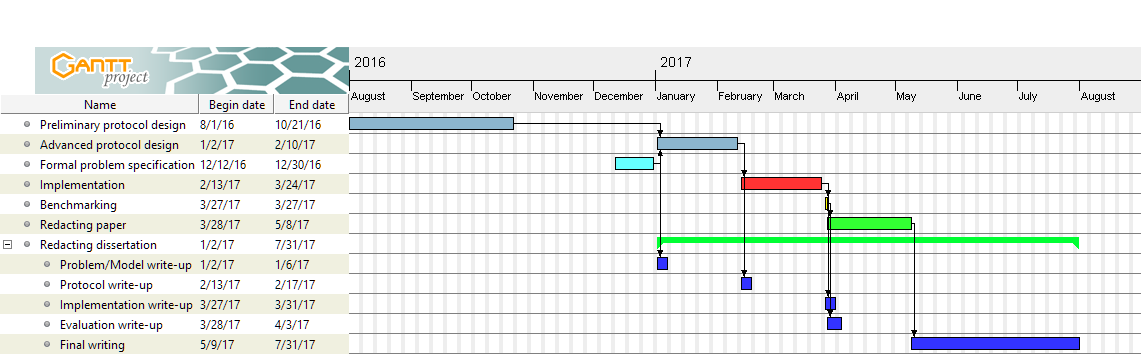
\includegraphics[width=\textwidth,height=\textheight,keepaspectratio]{Proposal}
	\caption{Gantt chart depicting proposed schedule}
	\label{fig:proposal}
	\centering
\end{figure}


\end{document}
